\documentclass[conference]{IEEEtran}
\IEEEoverridecommandlockouts
% The preceding line is only needed to identify funding in the first footnote. If that is unneeded, please comment it out.
\usepackage{cite}
\usepackage{amsmath,amssymb,amsfonts,amsthm}
\usepackage{graphicx}
\graphicspath{{figures/}}
\usepackage{textcomp}
\usepackage{xcolor}
\usepackage{fancyhdr}
\usepackage[hidelinks]{hyperref}
\usepackage{booktabs}
\usepackage{tikz}
\usetikzlibrary{arrows.meta,positioning,calc}

\def\BibTeX{{\rm B\kern-.05em{\sc i\kern-.025em b}\kern-.08em
    T\kern-.1667em\lower.7ex\hbox{E}\kern-.125emX}}

\newtheorem{proposition}{Proposition}
\newcommand{\Fcal}{\mathcal{F}}

\fancypagestyle{firstpage}{
  \fancyhf{}
  \fancyhead[C]{23rd Edition of IEEE India Council International Conference (INDICON 2026)}
  \fancyfoot[L]{%
      \begin{minipage}[t]{\textwidth}
      \normalsize{979-8-3195-2581-9/26/\$31.00\copyright2026 IEEE}
    \end{minipage}%
  }
  \renewcommand{\headrulewidth}{0pt}
}

\pagestyle{fancy}
\fancyhf{}
\fancyfoot[C]{INDICON 2026}
\renewcommand{\headrulewidth}{0pt}

\begin{document}

\title{Do Fractional Spectral Filters Help Fourier Neural Operators? A Controlled Ablation}

\author{\IEEEauthorblockN{Harshit Pranjal}
\IEEEauthorblockA{\textit{Dept. of Mathematics} \\
\textit{Birla Institute of Technology, Mesra}\\
Ranchi, India \\
imh10019.24@bitmesra.ac.in}
}

\maketitle
\thispagestyle{firstpage}

\begin{abstract}
Fourier neural operators (FNOs) learn solution maps of partial differential equations in Fourier space, but their spectral layers contain no explicit fractional-order structure. This paper tests whether a learnable, channel-wise spectral filter intended to encode fractional-order dissipation improves an FNO. It is shown analytically that a rational filter proposed in earlier work decays quadratically for every order and can be absorbed into the spectral weights, whereas the exact fractional propagator carries the order. These filters and a resolvent filter are compared in a controlled ablation on fractional Burgers, fractional Allen--Cahn and linear fractional diffusion, using five paired seeds, a fixed split, per-arm tuning, Holm correction, and U-Net and DeepONet baselines. With default settings the filters raise the Burgers error by a factor of 1.6--2.2 and lower the Allen--Cahn error by 42--78\%. After tuning, the Allen--Cahn gain vanishes at order 1.2 and persists at order 0.8, but it is not significant after correction and shrinks with longer training and more data. Learning the order adds nothing over a fixed filter, and the learned orders do not track the true order. A linear-response probe recovers the exponent of linear fractional diffusion from an unfiltered FNO with a mean absolute error of 0.072, so exponent recovery is not evidence for the filter. Negative and inconclusive outcomes are reported as such.
\end{abstract}

\begin{IEEEkeywords}
Fourier neural operator, fractional PDE, operator learning, spectral filter, ablation, fractional Laplacian
\end{IEEEkeywords}

\section{Introduction}
Neural operators learn mappings between function spaces and serve as fast surrogates for repeated PDE solves~\cite{kovachki2023neural,lu2021learning}. The Fourier neural operator (FNO) parameterizes an integral kernel in the Fourier domain at $\mathcal{O}(N\log N)$ cost per layer~\cite{li2021fourier,lu2022comprehensive}. Physics-informed methods instead embed the governing equation in the training loss~\cite{raissi2019physics,pang2019fpinns}.

Fractional PDEs describe anomalous diffusion and long-range interaction through the fractional Laplacian, whose Fourier symbol is $|k|^{\alpha}$ with $\alpha\in(0,2]$~\cite{podlubny1999fractional,metzler2000random,lischke2020fractional,kwasnicki2017ten}. A standard FNO layer learns unconstrained complex weights on a truncated set of modes and has no power-law structure built in. Inserting a learnable fractional spectral multiplier into the layer is therefore a natural idea~\cite{mehouachi2026fractional}. This paper asks whether such a multiplier improves accuracy once the comparison is controlled. The contributions are:
\begin{enumerate}
\item \textbf{Analysis.} The rational filter $1/(e^{1-\alpha}+\alpha k^2)$ decays as $k^{-2}$ for every $\alpha$, so $\alpha$ is a scale parameter and not a fractional order, whereas $\exp(-\beta|k|^{\alpha})$ encodes $\alpha$. Any positive filter is absorbable into the spectral weights, so it changes optimization and not expressivity.
\item \textbf{Controlled ablation.} Sixteen arms (Table~\ref{tab:arms}) are compared on three PDE systems with paired seeds, frozen-filter and initialization controls, pre-specified decision rules, per-arm tuning, longer training, more data, higher orders, Holm-corrected tests, and U-Net and DeepONet baselines.
\item \textbf{Probe and findings.} A linear-response probe recovers the dissipation exponent equally well from an unfiltered FNO. Filters degrade accuracy on Burgers and improve it on Allen--Cahn at default settings, but after tuning the Allen--Cahn gain vanishes at $\alpha=1.2$ and is not significant at $\alpha=0.8$.
\end{enumerate}

\section{Method}
\subsection{Filtered Fourier Layer}
Let $v_l$ be the latent field at layer $l$ with $C$ channels. A filtered Fourier layer computes
\begin{equation}
v_{l+1}=\sigma\!\left(W v_l+\Fcal^{-1}\!\left(R_\phi\,\Psi\,\Fcal v_l\right)\right),
\label{eq:layer}
\end{equation}
where $W\in\mathbb{R}^{C\times C}$ is a pointwise map, $R_\phi(k)\in\mathbb{C}^{C\times C}$ are learnable weights on the lowest $M$ modes, and $\Psi_i(k)$ is a filter applied to input channel $i$. Setting $\Psi\equiv 1$ gives the standard FNO. Wavenumbers are the integers $k\in\{0,\dots,M-1\}$ on the periodic domain $[0,2\pi)$. Fig.~\ref{fig:arch} shows the layer.

\begin{figure}[t]
\centering
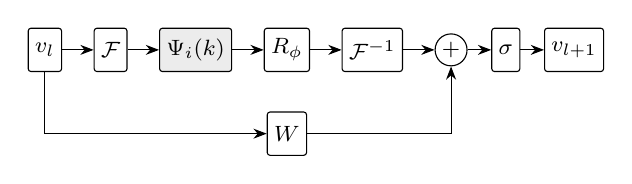
\begin{tikzpicture}[
  box/.style={draw,rounded corners=1pt,minimum height=0.55cm,inner sep=2.5pt,font=\footnotesize,align=center},
  >=Stealth, node distance=0.40cm]
\node[box] (v) {$v_l$};
\node[box,right=of v] (f) {$\Fcal$};
\node[box,right=of f,fill=gray!15] (psi) {$\Psi_i(k)$};
\node[box,right=of psi] (r) {$R_\phi$};
\node[box,right=of r] (fi) {$\Fcal^{-1}$};
\node[box,below=0.5cm of r] (w) {$W$};
\node[circle,draw,inner sep=1pt,right=of fi] (plus) {\footnotesize $+$};
\node[box,right=0.30cm of plus] (act) {$\sigma$};
\node[box,right=0.30cm of act] (vo) {$v_{l+1}$};
\draw[->] (v)--(f); \draw[->] (f)--(psi); \draw[->] (psi)--(r);
\draw[->] (r)--(fi); \draw[->] (fi)--(plus); \draw[->] (plus)--(act); \draw[->] (act)--(vo);
\draw[->] (v) |- (w); \draw[->] (w) -| (plus);
\end{tikzpicture}
\caption{Filtered Fourier layer. The shaded block is the channel-wise spectral filter $\Psi_i(k)$ applied before the spectral convolution.}
\label{fig:arch}
\end{figure}

\subsection{Filters}\label{sec:filters}
All adaptive filters use one parameter set per channel and block, with $\alpha_i=2\,\mathrm{sigmoid}(\hat\alpha_i)\in(0,2)$ initialized at $\alpha_i=1$, a $10\times$ learning rate and no weight decay. The \emph{rational filter} from earlier work is
\begin{equation}
\Psi_i(k)=\frac{1}{e^{1-\alpha_i}+\alpha_i k^{2}}.
\label{eq:rational}
\end{equation}
The \emph{fractional symbol} is the exact propagator form
\begin{equation}
\Psi_i(k)=\exp\!\left(-\beta_i\,|k|^{\alpha_i}\right),\qquad \beta_i=\mathrm{softplus}(\hat\beta_i)>0 .
\label{eq:power}
\end{equation}
For $\beta=\nu T$ this is the exact propagator of $u_t=-\nu(-\Delta)^{\alpha/2}u$ over time $T$. Arm A6 initializes $\beta=\ln 2$ and $\alpha=1$; arm A6i uses the scaled wavenumber $k/M$ and $\beta=10^{-3}$, so that $\Psi\approx 1$ at step zero. The \emph{Gaussian low-pass control} is
\begin{equation}
\Psi(k)=\exp\!\left(-\frac{k^2}{2\sigma^2}\right),
\label{eq:gauss}
\end{equation}
with $\sigma\in\{2,4,8,16\}$ chosen on the validation set. At initialization the adaptive filters are strongly low-pass on the retained modes: at $k=15$ the attenuation is 47\,dB for the rational filter at $\alpha=1$ (A5), 52\,dB for the fixed rational filter at $\alpha=1.8$ (A3) and 90\,dB for the fractional symbol with $\beta=\ln 2$ (A6). The spectral weights must compensate, which is why A6i was added.

\section{Theoretical Analysis}

\begin{proposition}[Fixed quadratic roll-off]\label{prop:decay}
For every $\alpha>0$ the rational filter~\eqref{eq:rational} satisfies $0<\Psi(k)\le e^{\alpha-1}$, decreases monotonically in $k\ge0$, and
\begin{equation}
\lim_{k\to\infty}\frac{\log\Psi(k)}{\log k}=-2 .
\label{eq:slope}
\end{equation}
\end{proposition}
\begin{proof}
The denominator is at least $e^{1-\alpha}>0$, which gives the bound, attained at $k=0$. The derivative is $-2\alpha k\,[e^{1-\alpha}+\alpha k^2]^{-2}<0$ for $k>0$, and $\Psi(k)=(\alpha k^2)^{-1}(1+o(1))$ for large $k$.
\end{proof}
By Proposition~\ref{prop:decay} and~\eqref{eq:slope}, $\alpha$ in~\eqref{eq:rational} sets a gain and a knee frequency, not a decay exponent. Fig.~\ref{fig:decay} (left) shows slope $-2$ for all $\alpha$.

\begin{proposition}[Exact fractional propagator]\label{prop:frac}
Let $u$ solve $u_t=-\nu(-\Delta)^{\alpha/2}u$ on the periodic domain. Then $\hat u(k,T)=\exp(-\nu T|k|^{\alpha})\,\hat u(k,0)$. Consequently $\log(-\log\Psi(k))=\log\beta+\alpha\log k$ for the symbol~\eqref{eq:power}, and the order $\alpha$ is the log--log slope of $-\log\Psi$.
\end{proposition}
\begin{proof}
The symbol of $(-\Delta)^{\alpha/2}$ is $|k|^{\alpha}$, so each mode obeys $\hat u_t=-\nu|k|^{\alpha}\hat u$. Taking logarithms twice gives the second statement.
\end{proof}
By Proposition~\ref{prop:frac}, a hand-constructed arm A6 with unit spectral weights reproduces the exact linear-diffusion solution to a relative error of $5.5\times10^{-6}$, so the hypothesis class contains the true operator for system S3.

\begin{figure}[t]
\centering
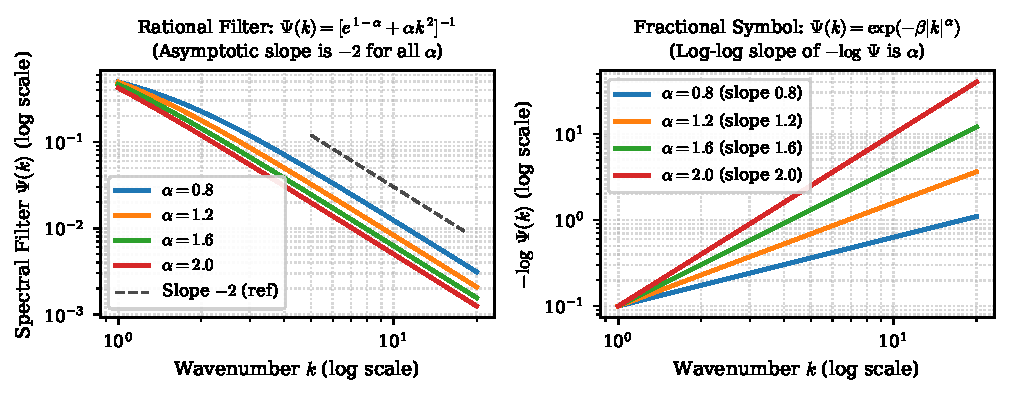
\includegraphics[width=0.98\columnwidth]{fig_spectral_decay_comparison.pdf}
\caption{Left: the rational filter has log--log slope $-2$ at large $k$ for every $\alpha$. Right: for the fractional symbol the quantity $-\log\Psi$ has slope $\alpha$.}
\label{fig:decay}
\end{figure}

\begin{proposition}[Hypothesis-class equivalence]\label{prop:absorb}
Let $\Psi_i(k)>0$ be fixed. The functions realizable by layer~\eqref{eq:layer} with filter $\Psi$ coincide with those realizable with $\Psi\equiv1$.
\end{proposition}
\begin{proof}
The filter scales input channel $i$ at mode $k$, so $[R_\phi(k)\Psi(k)]_{oi}=R_{oi}(k)\Psi_i(k)=:R'_{oi}(k)$, and $R\mapsto R'$ is a bijection of $\mathbb{C}^{C\times C}$ because $\Psi_i(k)>0$.
\end{proof}
By Proposition~\ref{prop:absorb}, a multiplicative filter therefore changes the optimization geometry and initial scale of the spectral weights and not the function class. Whether this reparametrization explains the effects in Section~\ref{sec:results} is not isolated by the experiments here.

\section{Linear-Response Spectral Probe}
To read off the dissipation a trained operator $\mathcal{G}_\Theta$ has learned, we perturb test inputs $a$ by $\varepsilon\sin(kx)$ and compute the gain $g(k)$ in~\eqref{eq:gain},
\begin{equation}
g(k)=\left\langle\frac{\bigl|\widehat{\mathcal{G}_\Theta(a+\varepsilon\sin kx)}(k)-\widehat{\mathcal{G}_\Theta(a)}(k)\bigr|}{\varepsilon\,|\widehat{\sin kx}(k)|}\right\rangle_{a},
\label{eq:gain}
\end{equation}
averaged over test inputs at $\varepsilon=10^{-3}$ and $2\times10^{-3}$ to check linearity. We then fit the model~\eqref{eq:fit},
\begin{equation}
\log g(k)=\log C-\beta_{\mathrm{eff}}\,k^{\alpha_{\mathrm{eff}}},
\label{eq:fit}
\end{equation}
over modes where gain times input energy exceeds $10^{-3}$ of its maximum. Applied to the exact propagator, the probe returns $\alpha_{\mathrm{eff}}=\alpha_{\mathrm{true}}$. It reads the learned map and is independent of the architecture.

\section{Experimental Protocol}

\subsection{Systems and Data}
All systems live on $[0,2\pi)$ with $N=256$ grid points and final time $T=1$. S1 is fractional Burgers, $u_t+uu_x+\nu(-\Delta)^{\alpha/2}u=0$ with $\nu=0.1$. S2 is fractional Allen--Cahn, $u_t+\epsilon^{2}(-\Delta)^{\alpha/2}u-u+u^3=0$ with $\epsilon^{2}=0.01$. S3 is linear fractional diffusion, $u_t+\nu(-\Delta)^{\alpha/2}u=0$ with $\nu=0.1$ and exact solution $\exp(-\nu|k|^{\alpha}T)$. S3 uses $\alpha\in\{0.8,1.2,1.6,1.9\}$; S1 and S2 use $\alpha\in\{0.8,1.2\}$ in the main study and $\{1.6,1.9\}$ in a high-order tier. Initial conditions are zero-mean Gaussian random fields with covariance $(-\Delta+9I)^{-2}$, standardized to unit variance and mapped to $0.5u_0$ (S1), $\tanh u_0$ (S2) and $u_0$ (S3). Nonlinear systems use Strang splitting with an exact spectral step for the fractional term, an RK4 step for the nonlinear terms, 2/3-rule dealiasing and $\Delta t=10^{-3}$ (S2). S1 targets are computed at $N=512$, $\Delta t=5\times10^{-4}$ and spectrally truncated to 256 points.

\emph{Solver accuracy.} For S2 and S3 the spatial error is below 0.13\%, and halving $\Delta t$ changes the S1 and S2 solutions by $2.2\times10^{-4}$ and $3.0\times10^{-4}$ (relative). S1 is less well resolved at low order: the relative difference between $N=512$ and $N=1024$ is 20.2\%$\pm$9.2\% at $\alpha=0.8$ and 2.9\%$\pm$1.9\% at $\alpha=1.2$, but only $4.2\times10^{-5}$ and $3.4\times10^{-5}$ at $\alpha=1.6$ and $1.9$. Low-order S1 results therefore describe learning the discretized $N=512$ map and not the continuous PDE.

\emph{Splits.} Test indices 1000--1199 (200 samples) and validation indices 900--999 (100 samples) are fixed. Training sets of 100, 500 or 900 samples are drawn by seed from indices 0--899. The seeds are 42, 123, 999, 2024 and 2025, shared by all arms.

\subsection{Arms, Training and Metric}
Table~\ref{tab:arms} lists the arms. All share one backbone: a lifting layer ($1\to64$), four Fourier layers of width 64 with $M=16$ modes and GELU, and a projection ($64\to128\to1$) with $287{,}361$ parameters. Training uses AdamW with learning rate $10^{-3}$, weight decay $10^{-4}$, a cosine schedule with minimum rate $10^{-5}$, 100 epochs, batch size 125 (50 for 100 samples) and the mean-squared-error loss. The primary metric is the relative $L^2$ error $\|u-\hat u\|_2/\|u\|_2$ over all 200 test samples. Raw MAPE is undefined where $u=0$, and the smallest $|u|$ reaches $2\times10^{-6}$ on S1 ($\alpha=1.2$), so we use two secondary metrics,
\begin{equation}
\mathrm{sMAPE}=\frac{100}{n}\sum \frac{2|u-\hat u|}{|u|+|\hat u|+\delta},\quad \delta=10^{-6},
\label{eq:smape}
\end{equation}
\begin{equation}
\mathrm{MAPE}_\varepsilon=\frac{100}{n}\sum\frac{|u-\hat u|}{|u|+\varepsilon},\quad \varepsilon=0.01\,(\mathrm{std}(u)+10^{-10}).
\label{eq:mapee}
\end{equation}
Differences from A0 use two-sided paired $t$-tests over seeds with 95\% $t$-intervals and Holm correction over the 24 tuned comparisons (eight arms against A0 in three cells). Standard deviations are sample standard deviations ($n-1$).

\begin{table}[t]
\caption{Arms. Extra parameters are trainable parameters beyond the 287,361 of A0; U-Net (287,360) and DeepONet (287,362) are separate architectures of similar size.}
\label{tab:arms}
\centering
\scriptsize
\setlength{\tabcolsep}{3pt}
\begin{tabular}{@{}lp{6.2cm}r@{}}
\toprule
Arm & Description & Extra \\
\midrule
A0 & Vanilla FNO & 0 \\
A1 & Parameter-matched FNO (projection width 132) & 264 \\
A2 & Gaussian low-pass~\eqref{eq:gauss}, $\sigma$ chosen on validation & 0 \\
A3 & Fixed rational filter, $\alpha^*$ chosen on validation ($0.4$, $1.6$, $1.2$ in the tuned cells) & 0 \\
A5 & Adaptive rational filter, channel-wise & 256 \\
A5-leg & Additive path $a_c\Psi(k)\hat v$, $a_c{=}3.5$ at init (replica of earlier code) & 256 \\
A6 / A6i & Fractional symbol, $\beta{=}\ln2$ init / identity init & 512 \\
A6j & Fractional symbol, $k/M$, $\beta{=}0.3$ init & 512 \\
A7 & Rational filter, $\alpha$ frozen at random values & 0 \\
A8a / A8b & Additive diagonal skip, $\Psi\equiv1$ / per-channel output gain & 256 \\
A9a & Plain FNO; weights scaled once at init by the rational filter & 0 \\
A10 & Resolvent filter $1/(1+\beta(k/M)^{\alpha})$, $\beta{=}0.3$, $\alpha{=}1$ init & 512 \\
U-Net & 1D U-Net, three levels, GELU & -- \\
DeepONet & Branch MLP on 256 sensors, trunk MLP on $x$ & -- \\
\bottomrule
\end{tabular}
\end{table}

\begin{figure}[t]
\centering
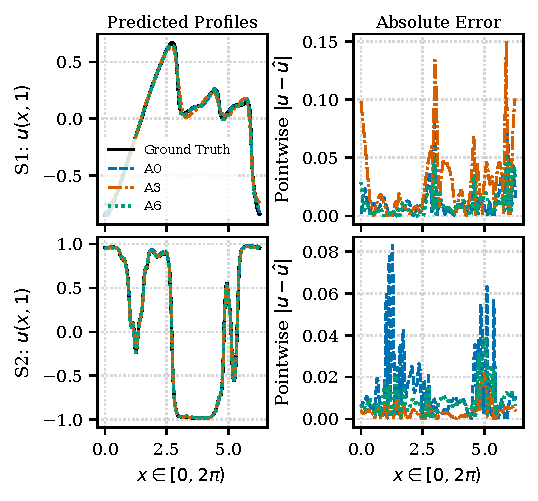
\includegraphics[width=0.75\columnwidth]{fig_qualitative.pdf}
\caption{Predicted vs Absolute Profiles for S1 \& S2.}
\label{fig:qualitative}
\end{figure}

\subsection{Decision Rules}
The following rules were fixed before the nonlinear runs. R1: the fractional symbol is a headline result only if it beats A0 and A2 by more than 10\% in relative $L^2$ on at least three of four orders and its recovered order has Spearman $\rho\ge0.8$. R2: if A2 is within 5\% of A6, the effect is reported as a spectral smoothing bias. R3: if A0 recovers the order as well as A6, the probe is a diagnostic only. R4: if A5-leg is within 5\% of A8 or A0 on at least three of four cells, the earlier gain is attributed to the additive near-identity path. R5: A6i helps in the nonlinear regime only if it beats A0 and A2 by more than 10\% on at least two of four cells. A6j, A9a, A10, U-Net, DeepONet, per-arm tuning, and the 300-epoch, 900-sample and high-order runs were added later and are exploratory.

\section{Results}\label{sec:results}

\subsection{Linear Fractional Diffusion (S3)}
Table~\ref{tab:s3} gives the test error with 500 training samples. The filters do not improve on the default FNO at any order: A5 is 1.4--2.9 times worse and A6 is 1.1--2.2 times worse. R1 is not met and R3 is triggered.

\begin{table}[t]
\caption{S3 relative $L^2$ error ($\times10^{-2}$), mean $\pm$ std over 5 seeds, 500 training samples.}
\label{tab:s3}
\centering
\scriptsize
\setlength{\tabcolsep}{3pt}
\begin{tabular}{@{}lcccc@{}}
\toprule
Arm & $\alpha{=}0.8$ & $\alpha{=}1.2$ & $\alpha{=}1.6$ & $\alpha{=}1.9$ \\
\midrule
A0 & $\mathbf{1.51\pm0.05}$ & $\mathbf{1.19\pm0.05}$ & $1.40\pm0.06$ & $\mathbf{1.32\pm0.06}$ \\
A1 & $\mathbf{1.51\pm0.07}$ & $\mathbf{1.19\pm0.04}$ & $\mathbf{1.39\pm0.04}$ & $\mathbf{1.32\pm0.04}$ \\
A2 & $1.53\pm0.05$ & $1.51\pm0.05$ & $1.42\pm0.06$ & $1.34\pm0.06$ \\
A5 & $2.15\pm0.07$ & $3.41\pm0.10$ & $2.89\pm0.41$ & $1.90\pm0.19$ \\
A6 & $1.92\pm0.08$ & $2.56\pm0.18$ & $1.83\pm0.07$ & $1.50\pm0.03$ \\
\bottomrule
\end{tabular}
\end{table}

Table~\ref{tab:alpha} and Fig.~\ref{fig:alphaeffective} give the probed exponent. The mean absolute error (MAE) is taken over the four per-order means, so that the four physical conditions are the units and the 20 runs are not treated as independent. A0, which has no fractional parameter, has the lowest error (0.072) and the correct rank order. A6 is worse (0.198) and its estimate at $\alpha=1.2$ varies strongly between seeds ($0.974\pm0.40$). A5 does not track the order (0.699). Because an unfiltered FNO recovers the exponent, exponent recovery shows that the learned map fits the data, not that the filter discovered the physics.

\begin{table}[t]
\caption{Probed exponent $\alpha_{\mathrm{eff}}$ on S3, mean over 5 seeds. MAE is over the four per-order means.}
\label{tab:alpha}
\centering
\scriptsize
\setlength{\tabcolsep}{4pt}
\begin{tabular}{@{}lcccc@{}}
\toprule
$\alpha_{\mathrm{true}}$ & A0 & A2 & A5 & A6 \\
\midrule
0.8 & 0.924 & 0.928 & 0.342 & 0.437 \\
1.2 & 1.278 & 1.337 & 0.231 & 0.974 \\
1.6 & 1.646 & 1.646 & 0.527 & 1.756 \\
1.9 & 1.941 & 1.941 & 2.195 & 1.946 \\
\midrule
MAE & \textbf{0.072} & 0.088 & 0.699 & 0.198 \\
\bottomrule
\end{tabular}
\end{table}

\begin{figure}[t]
\centering
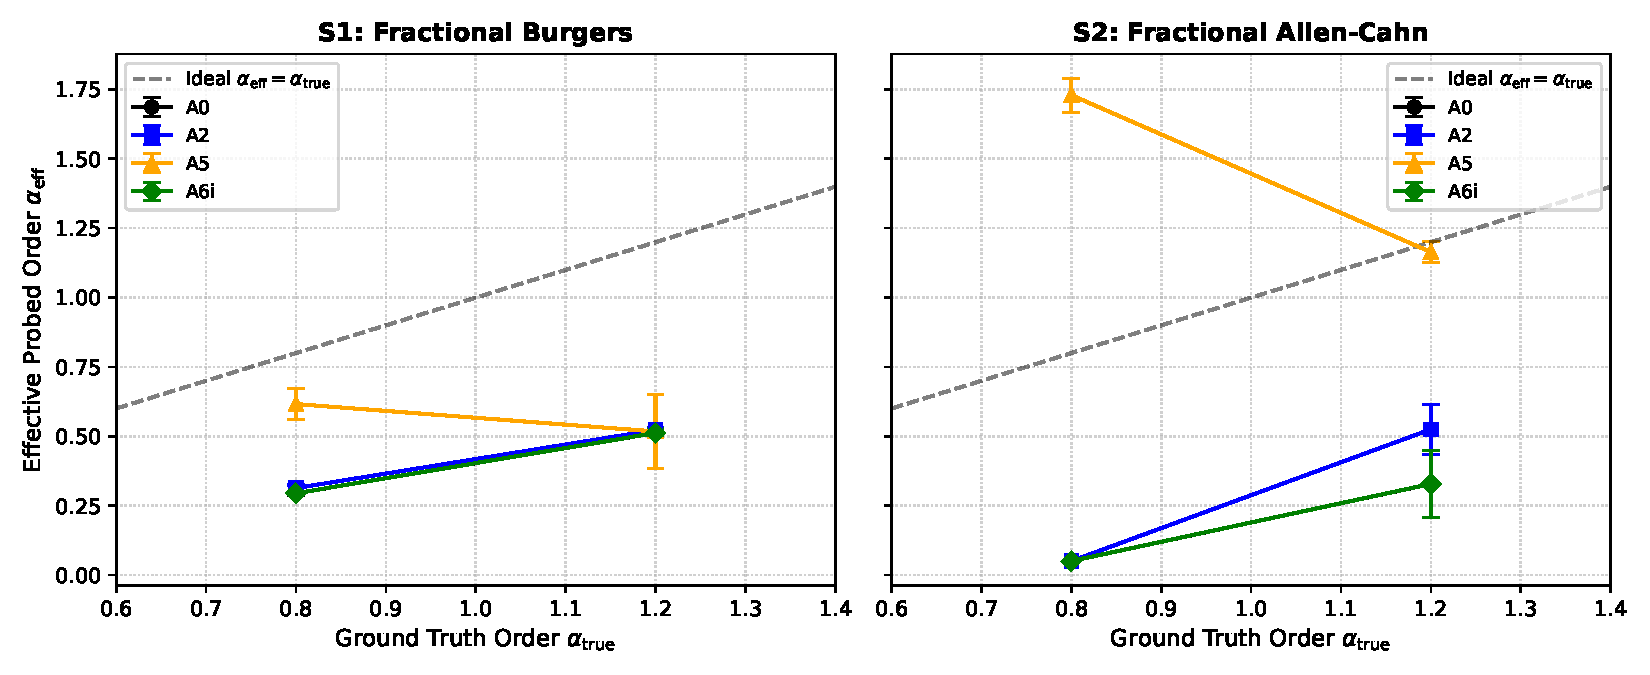
\includegraphics[width=0.98\columnwidth]{alpha_eff.pdf}
\caption{Effective order of $\alpha$ probed across systems.}
\label{fig:alphaeffective}
\end{figure}

\subsection{Nonlinear Systems (S1, S2)}
Table~\ref{tab:core} reports all arms with default settings and 500 training samples, with representative predicted profiles and absolute errors in Fig.~\ref{fig:qualitative} and training trajectories in Fig.~\ref{fig:curves}.
\textbf{Default settings.} On Burgers, A3, A5 and A7 raise the error of A0 by a factor of 1.6--2.2, the additive skip A8a by 1.8--2.7, and A6 by 7--8\%; A8b is within 2\% of A0. On Allen--Cahn every filtered variant (A3, A5, A6, A7) reduces the error of A0 by 42--78\%, with the best arm A3 at $\alpha=0.8$ and A6 at $\alpha=1.2$. The parameter-matched A1, the Gaussian control A2 and the output gain A8b do not reproduce this. At $\alpha=1.6$ and $1.9$ (Table~\ref{tab:extra}) no filter improves accuracy: A3 is 53\% and 74\% worse than A0 on Burgers, and all arms lie within 11\% of A0 on Allen--Cahn. The gain is therefore confined to low orders.

\begin{table*}[t]
\caption{Core ablation under default hyperparameters ($N_{\mathrm{tr}}=500$, 100 epochs, relative $L^2$ error, mean $\pm$ sample std over 5 seeds). Bold marks the lowest error per column.}
\label{tab:core}
\centering
\scriptsize
\setlength{\tabcolsep}{6pt}
\begin{tabular}{lcccc}
\toprule
 & \multicolumn{2}{c}{S1 Burgers} & \multicolumn{2}{c}{S2 Allen--Cahn} \\
\cmidrule(lr){2-3}\cmidrule(lr){4-5}
Arm & $\alpha=0.8$ & $\alpha=1.2$ & $\alpha=0.8$ & $\alpha=1.2$ \\
\midrule
A0 & $0.1085\pm0.0070$ & $0.0549\pm0.0060$ & $0.0399\pm0.0031$ & $0.0321\pm0.0013$ \\
A1 & $0.1101\pm0.0039$ & $0.0546\pm0.0033$ & $0.0370\pm0.0030$ & $0.0301\pm0.0015$ \\
A2 & $0.1099\pm0.0063$ & $0.0551\pm0.0062$ & $0.0391\pm0.0031$ & $0.0312\pm0.0014$ \\
A3 & $0.1728\pm0.0071$ & $0.1054\pm0.0052$ & $\mathbf{0.0086\pm0.0013}$ & $0.0187\pm0.0010$ \\
A5 & $0.1772\pm0.0113$ & $0.1120\pm0.0090$ & $0.0110\pm0.0005$ & $0.0177\pm0.0009$ \\
A5-leg & $1.0155\pm0.1611$ & $1.0352\pm0.1852$ & $0.5413\pm0.0632$ & $0.5734\pm0.0657$ \\
A6 & $0.1156\pm0.0052$ & $0.0591\pm0.0058$ & $0.0105\pm0.0028$ & $\mathbf{0.0173\pm0.0010}$ \\
A6i & $0.1085\pm0.0070$ & $0.0549\pm0.0060$ & $0.0399\pm0.0031$ & $0.0321\pm0.0013$ \\
A7 & $0.1962\pm0.0083$ & $0.1230\pm0.0069$ & $0.0112\pm0.0006$ & $0.0177\pm0.0009$ \\
A8a & $0.1960\pm0.0079$ & $0.1484\pm0.0116$ & $0.1035\pm0.0052$ & $0.0939\pm0.0050$ \\
A8b & $\mathbf{0.1073\pm0.0067}$ & $\mathbf{0.0540\pm0.0060}$ & $0.0399\pm0.0032$ & $0.0320\pm0.0013$ \\
\bottomrule
\end{tabular}
\end{table*}

\textbf{Adaptivity.} A5 and the frozen A7 agree within 2\% on Allen--Cahn, and the validation-tuned fixed filter A3 beats the adaptive A5 in three of four cells, so learning the order adds little. The learned orders do not track the PDE: the mean final $\alpha$ of A5 over five seeds is $0.838\pm0.018$ on Burgers ($\alpha_{\mathrm{true}}=1.2$), $1.018\pm0.006$ on Allen--Cahn at $\alpha_{\mathrm{true}}=0.8$ and $1.013\pm0.008$ at $1.2$, from an initial value of 1. The values are reproducible across seeds but nearly equal for the two Allen--Cahn orders, so $\alpha$ acts as a numerical filter scale and not a physical order.

\textbf{Earlier additive variant.} The replica of the earlier additive path (A5-leg) gives errors of $0.54$--$1.04$ on every cell, far above A0 and A8a, so R4 is not met. Its initial gain is $a_c\Psi\approx7.8$ in each of four blocks and training is unstable. The earlier implementation used a single Fourier layer, so this result describes the additive path in a four-block FNO and not the earlier network itself.

\textbf{Identity initialization.} A6i equals A0 to four decimals in all 20 runs and at 300 epochs, so R5 fails on all four cells. For seed 42, $\beta$ ends at about $10^{-3}$ and $\alpha$ within 0.03 of 1: since $\beta=\mathrm{softplus}(\hat\beta)$ with $\hat\beta\approx-6.9$, the factor $\partial\beta/\partial\hat\beta\approx10^{-3}$ reduces the gradient of $\hat\beta$ to $10^{-7}$--$10^{-6}$. The outcome is uninformative about identity-initialized fractional filters. The gap between A6 ($0.0105$) and A6i ($0.0399$) at $\alpha=0.8$ on Allen--Cahn shows that the effect comes from the strongly attenuating initial symbol.

\begin{figure}[t]
\centering
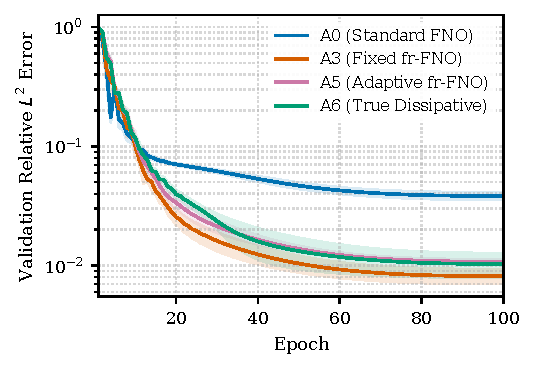
\includegraphics[width=0.75\columnwidth]{fig_curves.pdf}
\caption{Relative $L^2$ Error across all benchmarks}
\label{fig:curves}
\end{figure}

\subsection{Per-Arm Tuning and Other Operators}\label{sec:tuned}
The default settings undertrain every arm, so each arm was tuned separately (Table~\ref{tab:tuned}). For each arm and cell, learning rate $\{3\times10^{-4},10^{-3},3\times10^{-3}\}$ and weight decay $\{0,10^{-4}\}$ were scored on the validation set (100 epochs, seed 42), and the best pair was run for all five seeds; the test set was not used for selection. The selected pair was $(3\times10^{-3},0)$ for every model in every cell except A6 on S2 at $\alpha=1.2$ (weight decay $10^{-4}$), so the optimum lies on the upper edge of the grid. Tuning improves every arm: A5 on Burgers falls from 0.1120 to 0.0554, A3 from 0.1054 to 0.0575, and A0 on Allen--Cahn at $\alpha=0.8$ from 0.0399 to 0.0128.

\begin{table}[t]
\caption{Tuned comparison, 500 training samples, 100 epochs, mean $\pm$ sample std over 5 seeds. Bold marks the lowest value per column.}
\label{tab:tuned}
\centering
\scriptsize
\setlength{\tabcolsep}{2.2pt}
\begin{tabular}{@{}lccc@{}}
\toprule
 & S1, $\alpha{=}1.2$ & S2, $\alpha{=}0.8$ & S2, $\alpha{=}1.2$ \\
\midrule
A0 & $0.0389\pm0.0063$ & $0.0128\pm0.0038$ & $0.0151\pm0.0012$ \\
A9a & $\mathbf{0.0382\pm0.0060}$ & $0.0127\pm0.0034$ & $0.0151\pm0.0010$ \\
A6j & $0.0392\pm0.0060$ & $0.0126\pm0.0042$ & $0.0151\pm0.0016$ \\
A10 & $0.0392\pm0.0060$ & $0.0126\pm0.0042$ & $0.0151\pm0.0016$ \\
A6 & $0.0399\pm0.0048$ & $\mathbf{0.0070\pm0.0011}$ & $0.0164\pm0.0007$ \\
A5 & $0.0554\pm0.0100$ & $0.0079\pm0.0008$ & $\mathbf{0.0148\pm0.0004}$ \\
A3 & $0.0575\pm0.0075$ & $0.0078\pm0.0005$ & $0.0161\pm0.0005$ \\
U-Net & $0.1674\pm0.0043$ & $0.0447\pm0.0054$ & $0.0443\pm0.0068$ \\
DeepONet & $0.4518\pm0.0090$ & $0.5375\pm0.0121$ & $0.5397\pm0.0214$ \\
\bottomrule
\end{tabular}
\end{table}

\begin{table*}[t]
\centering
\scriptsize
\setlength{\tabcolsep}{5pt}
\caption{Additional settings, relative $L^2$ error, mean $\pm$ sample std. 300 epochs: tuned, three seeds. $N_{\mathrm{tr}}=900$ and $\alpha\in\{1.6,1.9\}$: five seeds, 100 epochs, 900 and 500 training samples. Bold marks the lowest value per row; ``--'' means not run.}
\label{tab:extra}
\begin{tabular}{llccccc}
\toprule
Setting & Cell & A0 & A3 & A5 & A6 & A10 \\
\midrule
300 epochs & S1, $\alpha{=}1.2$ & $0.0269\pm0.0031$ & $0.0269\pm0.0025$ & $0.0211\pm0.0019$ & $\mathbf{0.0185\pm0.0007}$ & $0.0259\pm0.0028$ \\
300 epochs & S2, $\alpha{=}0.8$ & $0.0040\pm0.0003$ & $0.0044\pm0.0009$ & $0.0039\pm0.0002$ & $\mathbf{0.0035\pm0.0002}$ & $0.0040\pm0.0006$ \\
300 epochs & S2, $\alpha{=}1.2$ & $0.0107\pm0.0003$ & $0.0125\pm0.0001$ & -- & $0.0115\pm0.0001$ & $\mathbf{0.0107\pm0.0001}$ \\
$N_{\mathrm{tr}}{=}900$ & S1, $\alpha{=}1.2$ & $0.0233\pm0.0027$ & $0.0337\pm0.0024$ & -- & $\mathbf{0.0220\pm0.0005}$ & $0.0236\pm0.0026$ \\
$N_{\mathrm{tr}}{=}900$ & S2, $\alpha{=}0.8$ & $0.0055\pm0.0013$ & $0.0052\pm0.0011$ & -- & $\mathbf{0.0047\pm0.0008}$ & $0.0051\pm0.0011$ \\
High order & S1, $\alpha{=}1.6$ & $\mathbf{0.0225\pm0.0008}$ & $0.0345\pm0.0017$ & -- & $0.0228\pm0.0014$ & $0.0238\pm0.0013$ \\
High order & S1, $\alpha{=}1.9$ & $\mathbf{0.0181\pm0.0009}$ & $0.0315\pm0.0016$ & -- & $0.0182\pm0.0009$ & $0.0182\pm0.0010$ \\
High order & S2, $\alpha{=}1.6$ & $\mathbf{0.0249\pm0.0009}$ & $0.0255\pm0.0010$ & -- & $0.0253\pm0.0010$ & $0.0253\pm0.0008$ \\
High order & S2, $\alpha{=}1.9$ & $\mathbf{0.0182\pm0.0069}$ & $0.0185\pm0.0071$ & -- & $0.0201\pm0.0071$ & $0.0184\pm0.0069$ \\
\bottomrule
\end{tabular}
\end{table*}

\textbf{Burgers, $\alpha=1.2$.} At 100 epochs A0, A6, A6j, A10 and A9a lie within 4\% of each other (0.0382--0.0399). A3 and A5 are worse by 48\% and 42\%, but with Holm-adjusted $p=0.079$ and $0.36$ this is not significant. At 300 epochs (Table~\ref{tab:extra}) A3 ties A0, A5 is 22\% lower ($p=0.12$), and A6 is best at $0.0185$, 31\% below A0 (paired difference $-0.0083$, 95\% interval $[-0.0156,-0.0011]$, $p=0.035$). With three seeds and eight 300-epoch comparisons this does not survive Holm correction and is exploratory, but it shows that the 100-epoch disadvantage does not persist. At 900 samples A6 ties A0 while A3 stays 45\% worse ($p=0.003$, uncorrected).

\textbf{Allen--Cahn, $\alpha=1.2$.} All FNO arms lie between 0.0148 and 0.0164 with overlapping intervals. At 300 epochs A0 reaches $0.0107$, A10 matches it, and A6 and A3 are 8\% and 17\% worse. No filter gain survives at this order.

\textbf{Allen--Cahn, $\alpha=0.8$.} At 100 epochs the strongly attenuating filters keep an advantage: A6 ($0.0070$), A3 ($0.0078$) and A5 ($0.0079$) are 38--45\% below A0 ($0.0128$), whose error varies strongly across seeds. Uncorrected paired $t$-tests give $p=0.030$ (A6), $0.036$ (A5) and $0.040$ (A3), and Holm-adjusted values over the 24 comparisons are $0.47$, $0.54$ and $0.55$. All three arms beat A0 on all five seeds, but with $n=5$ the smallest attainable two-sided exact Wilcoxon $p$ is $1/16=0.0625$, so neither test can reach 0.05. The result is suggestive and not established. The near-identity filters A6j, A10 and the rescaled-initialization control A9a ($0.0126$--$0.0127$) do not improve accuracy, so the effect needs a strongly attenuating filter that remains in the forward pass. The advantage also shrinks with training length and data: at 300 epochs the arms are at parity (A0 $0.0040$, A6 $0.0035$, paired difference $-0.0004$, $p=0.054$), and at 900 samples A6 is 15\% below A0 ($p=0.089$) with A3 and A10 5--7\% below, none significant.

\textbf{Adaptivity and near-identity filters.} A5 and the fixed A3 tie in all three tuned cells, so adapting the order adds nothing. For the tuned A6 (seed 42) the mean final $\alpha$ is $0.97$ on S2 ($\alpha_{\mathrm{true}}=0.8$) and $0.71$ on S1 ($\alpha_{\mathrm{true}}=1.2$), so the fractional symbol does not recover the physical order either. A6j and A10 barely move from initialization ($\alpha$ ends at $0.96$--$0.99$ and $\beta$ at $0.29$--$0.32$). They are separate implementations, $\exp(-\beta(k/M)^{\alpha})$ and $1/(1+\beta(k/M)^{\alpha})$, with the same first-order expansion, yet their errors agree to four decimals in every cell. We could not fully explain this, so they are counted as one weak test of an $\alpha$-controlled filter.

\textbf{Other operators.} The U-Net has 2.9--4.3 times the error of the tuned FNO and DeepONet 12--42 times. These six comparisons against A0 are the only ones that survive Holm correction (adjusted $p\le1.9\times10^{-3}$). DeepONet underfits: on S2 ($\alpha=0.8$, seed 42) its training error is $0.570$ and its test error $0.561$. Of four modifications (input normalization, trunk Fourier features $k=1,\dots,16$, width 256, 300 epochs), Fourier features gave the largest improvement (test $0.250$, training $0.145$), reaching $0.249\pm0.003$ on S1 ($\alpha=1.2$) and $0.255\pm0.004$ on S2 ($\alpha=0.8$) over five seeds; the others stay between $0.42$ and $0.54$. Even this variant is 6.4 and 20 times worse than the tuned A0, so DeepONet remains a weak reference and no general claim about it is made.

\textbf{Training length and data size.} The 300-epoch runs improve every arm; on S2 at $\alpha=1.2$ the U-Net reaches $0.0200$ and DeepONet $0.432$. With default settings on S1 ($\alpha=1.2$), A0 improves from $0.0570$ to $0.0256$ at 300 epochs and the A5 excess over A0 narrows from 92\% to 32\%. With 100 training samples and default settings the filters again degrade accuracy on Burgers (A5 $0.1800$ and A6 $0.1415$ vs.\ A0 $0.1083$), while on Allen--Cahn A5 and A6 cut the A0 error by 57--60\% at 100 samples and by 45--46\% at 500. A tuned baseline at 100 samples was not run, so no sample-efficiency claim is made.

\textbf{Secondary metrics.} The sMAPE~\eqref{eq:smape} and MAPE$_\varepsilon$~\eqref{eq:mapee} of the tuned arms rank them as relative $L^2$ does in every cell. For example, on S2 ($\alpha=0.8$) A0 has 2.81\% and 2.42\% against 1.44\% and 1.14\% for A6, and on S1 ($\alpha=1.2$) A0 has 7.97\% and 7.25\% against 10.59\% and 10.47\% for A3. The clamped raw MAPE over $|u|\ge10^{-4}$ is 1.3--1.8 times the sMAPE for FNO arms and reaches 185\% for DeepONet.

\textbf{Cost and resolution transfer.} On one Apple GPU, the filters add 3--20\% to the training time per epoch (A0 0.117\,s, A6j 0.141\,s) and change the inference latency by less than 12\%, within the noise of single measurements; DeepONet trains about ten times faster. Models trained at $N=256$ and evaluated at $N\in\{64,128,512\}$ ($\alpha=1.2$, five seeds) stay within 6\% of their native error for $N\ge128$ and differ by 7--40\% at $N=64$ (largest for A5 on S2, $0.0247$ vs.\ $0.0177$). The ranking of A0 and A5 is the same at every resolution, so the filter neither removes nor clearly improves the degradation at the coarsest grid.

\section{Limitations}
(i) Hyperparameters were selected on one seed from six pairs, and the selected learning rate was the largest in the grid, so a wider grid could change the ranking. (ii) The Allen--Cahn advantage at $\alpha=0.8$ does not survive Holm correction, and the 300-epoch, 900-sample, Burgers and high-order results use three or five seeds and are exploratory; an exact Wilcoxon test cannot reach $p<0.05$ with five seeds. (iii) The mechanism is not isolated: rescaling the initial weights (A9a) does not reproduce the effect, which points to the persistent filter, but a persistent reparametrization of the spectral weights remains a hypothesis. (iv) A6i never left its initial values, and A6j and A10 form one weak test. (v) The Burgers $\alpha=0.8$ reference is not converged. (vi) The study covers three systems, four orders and one network width; a fractional Fisher--KPP system was designed and its solver verified, but no networks were trained on it. (vii) DeepONet underfits at this size, and the U-Net is one architecture.

\section{Conclusion}
A learnable spectral filter does not make an FNO learn fractional order. The rational filter cannot encode an order by construction, the learned orders do not track the true order, the exact fractional symbol and the resolvent filter did not beat a fixed or tuned filter, and an unfiltered FNO recovers the exponent of linear fractional diffusion at least as well. With default settings, filters degrade accuracy on Burgers and improve it on Allen--Cahn. After per-arm tuning the Allen--Cahn gain vanishes at $\alpha=1.2$ and at high orders, and at $\alpha=0.8$ it is not significant after Holm correction and shrinks with longer training and more data. The FNO family clearly beats a U-Net and a DeepONet of the same size. Practitioners should compare against a tuned, fully trained vanilla FNO, and against frozen and initialization controls, before attributing a gain to fractional structure.

\section*{Data and Code Availability}
All datasets, scripts and per-run records are available at \url{https://github.com/HarshitPranjal/Fractional-FNO-Fr-FNO-}.

\bibliographystyle{IEEEtran}
\bibliography{References}

\end{document}
